
\section{Experiments}\label{sect:experiments}

In this section, we evaluate \fname{} against both PPO (for single agent settings), MAPPO (for multi-agent settings), and SHAC across various multi-agent scenarios and architectures. An ablation study replacing only the transition function (SHAC+, where the reward function remains differentiable) is provided in \Cref{apx:ablation}.
We select PPO as our baseline because, despite the emergence of more recent algorithms HAPPO \cite{Kuba2021TrustRM}, and SAC \cite{Haarnoja2018SoftAA}, it remains one of the few approaches that scales effectively to multi-agent settings without substantial modifications (e.g., MAPPO~\cite{DBLP:conf/nips/YuVVGWBW22}). This makes PPO a representative benchmark for state-of-the-art performance in non-differentiable environments.

\paragraph{Scenarios}
We evaluate our algorithms on several multi-agent scenarios from VMAS~\cite{DBLP:conf/dars/BettiniKBP22}, which we selected over alternatives like PettingZoo~\cite{DBLP:conf/icml/PettingZoo}, SMAC~\cite{DBLP:conf/icml/ZhangZLZ20}, MA-MuJoCo~\cite{DBLP:conf/aaai/GuptaK0G20}, and others due to its key advantages: differentiable physics (enabling gradient-based optimization), multi-agent design, vectorized implementation (for efficient parallel training), realistic physics-based simulation, and open-source accessibility.
For more details about the choice of environments, see \Cref{apx:scenarios}.
We selected four distinct scenarios: Dispersion, Discovery, Transport, and Sampling, specifically for their cooperative nature and varying levels of required coordination (see \Cref{fig:scenarios} and \Cref{apx:scenarios} for details). These scenarios can be categorized along two dimensions:
\begin{compactitem}
    \item \textbf{Reward differentiability:} Dispersion and Discovery feature non-differentiable reward functions (making SHAC inapplicable), while Transport and Sampling have differentiable rewards (allowing for SHAC implementation).
    \item \textbf{Observation completeness:} Transport and Dispersion provide agents with complete observation spaces relative to the environment state. In contrast, Discovery and Sampling have incomplete observation spaces, which presents an additional challenge for \fname{} compared to SHAC, as \fname{} lacks access to the complete environmental state.
\end{compactitem}

\noindent This selection of scenarios enables a thorough evaluation of how each algorithm handles different types of multi-agent cooperation challenges.

\paragraph{Architectures}
We test SHAC, PPO, and \fname{} with both an MLP and a Transformer architecture. Specifically, we use a 1-layer MLP or a 1-layer single-head Transformer for policy, reward, and value network. The transition network used by \fname{} is always a 3-layer single-head Transformer

While the MLP architecture is the simplest, the Transformer baseline benefits from positional invariance property of the agents observations. We apply the transformer architecture only if the number of agents is greater than $1$, otherwise we use only the MLP architecture. For more details on the architectures, see \Cref{apx:arch}.

\paragraph{Hyperparameters}
For all networks we use learning rate of $1e\text{-}3$ with Adam Optimizer~\cite{Kingma14}. For all scenarios, each training episode consists of $512$ environments of $32$ steps each. Each validation episode is composed of $512$ environments of $512$ steps each. We employ early stopping when the agents achieve $90\%$ of the maximum reward in $90\%$ of the episode's environments. If early stopping is not triggered, we stop training after $20,000$ episodes. The discount factor is set to $0.99$ and lambda factor is set to $0.95$. We report results for increasing number of agents $n\in\{1,3,5\}$. We repeat and report results for $3$ runs with different seeds. See \Cref{apx:tab:ppo} and \Cref{apx:tab:shac} for a complete list of hyperparameters. Hyperparameter choices are the result of a small grid search on the transport scenario.

Overall, considering different training algorithms, architectures, scenarios, hyperparameters, we completed a total of $254$ runs lasting between $1$ to $8$ hours each. 

\paragraph{Hardware Setup}
All experiments were conducted on a cluster with two nodes, each equipped with a V100 GPU (32GB of memory) and 200GB of RAM, and one node with four A100 GPUs (40GB of memory) and 512GB of RAM. 

\begin{figure}
    \centering
    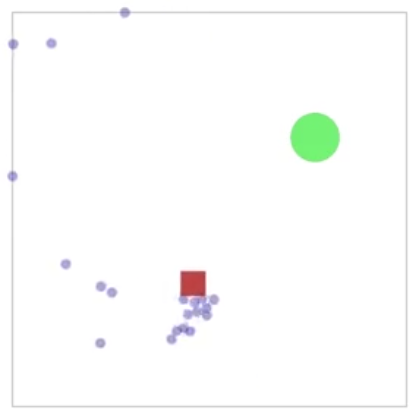
\includegraphics[width=0.32\columnwidth]{figs/step-1.png}
    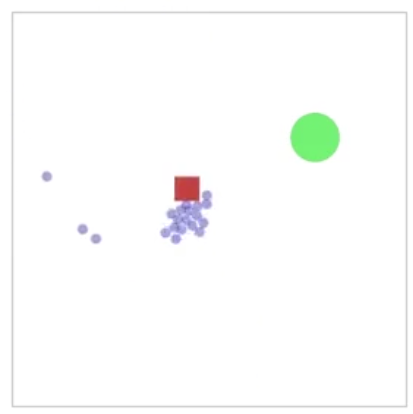
\includegraphics[width=0.32\columnwidth]{figs/step-2.png}
    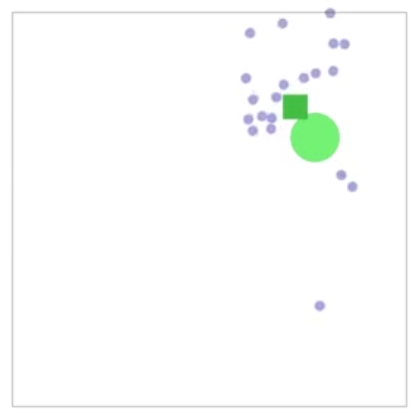
\includegraphics[width=0.32\columnwidth]{figs/step-3.png}
    \caption{Snapshots of trained agents with \fname{} in the Transport scenario. Colored circles represent agents pushing a red package (square) toward the green goal.}\label{fig:transport-trained}
\end{figure}

\begin{figure}
    \centering
    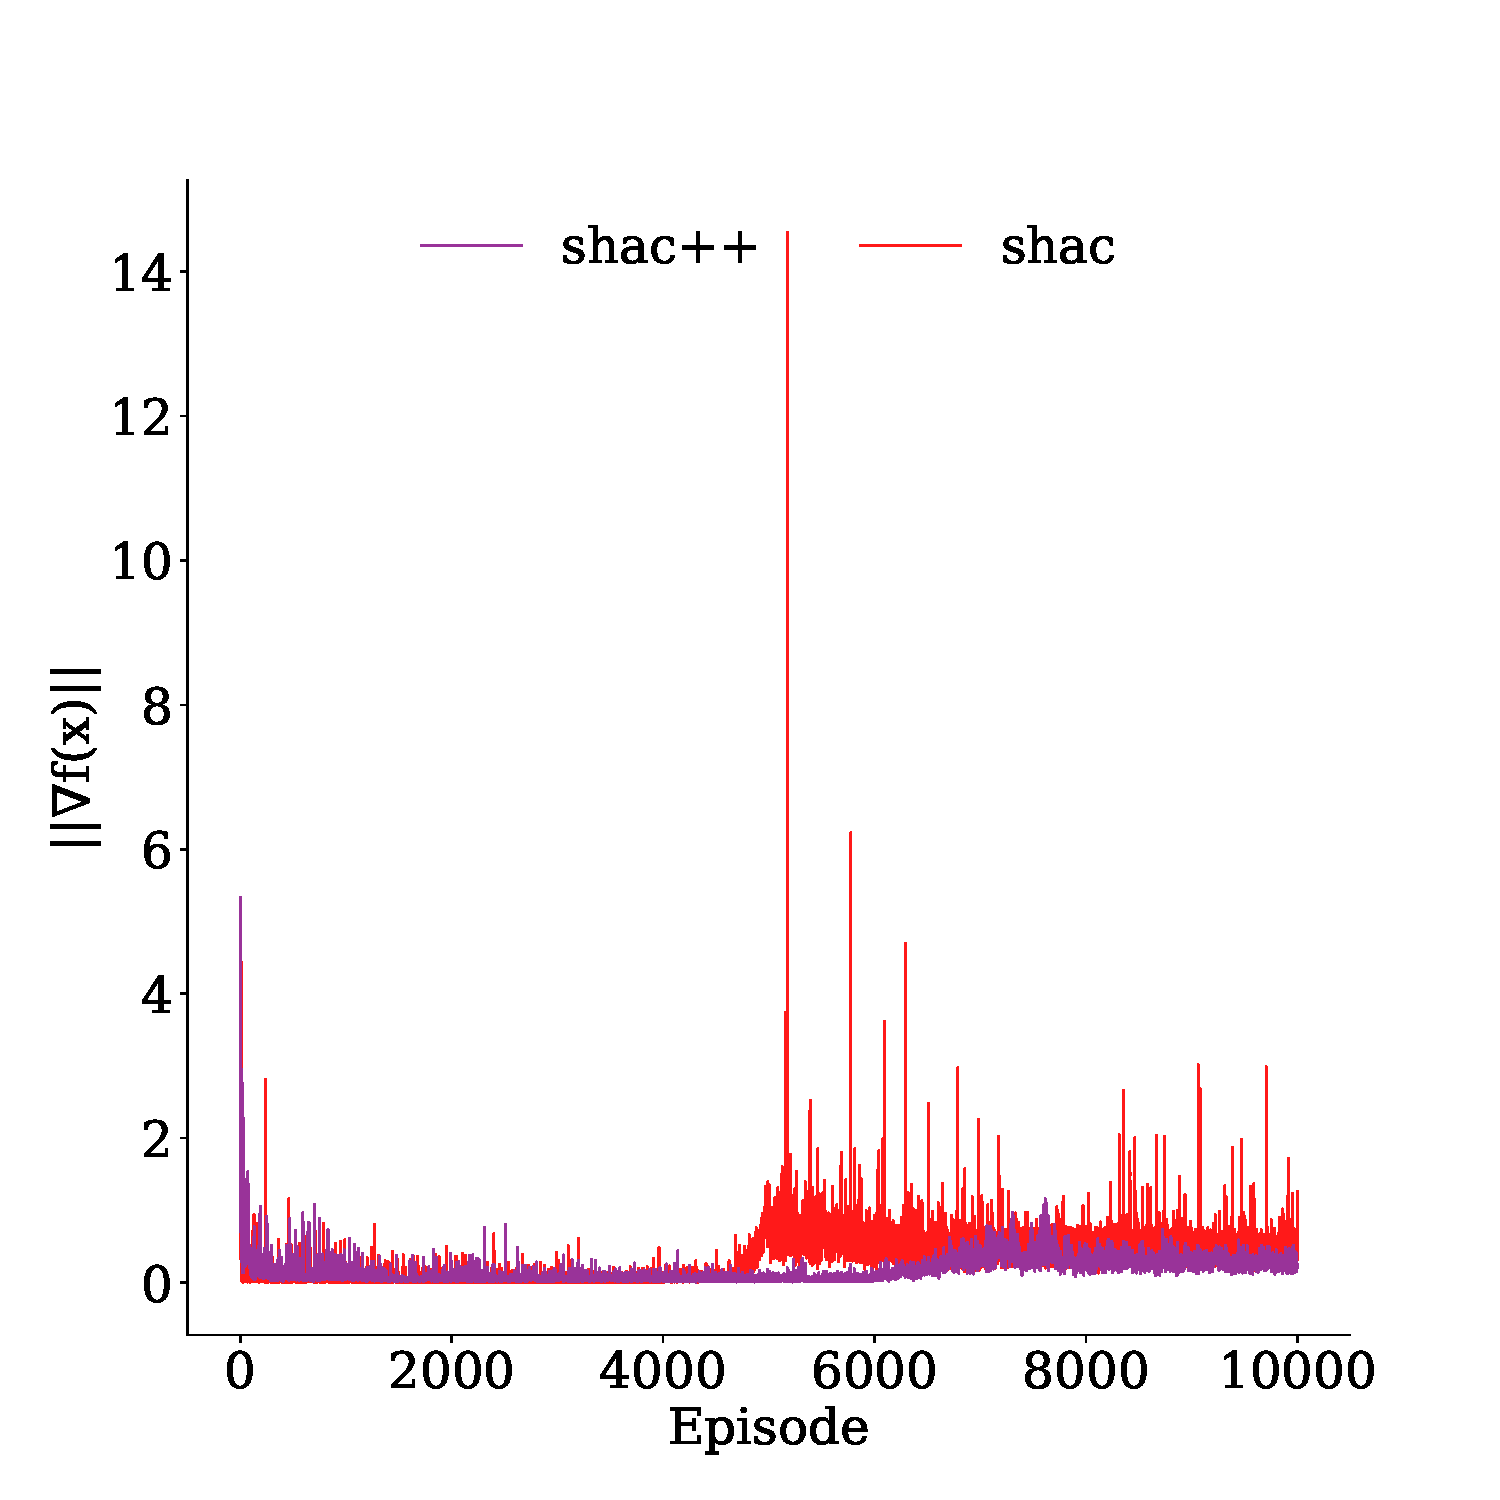
\includegraphics[width=0.7\columnwidth]{figs/grads-transformer-transport.pdf}
    \caption{Policy gradient norms in the Transport environment over 5000 epochs. Spikes in gradient norm for SHAC (epoch 2700) and \fname{} (epoch 3200) correspond to generalization events when agents begin frequent interactions with the package and each other.}\label{fig:grads-transformer-transport}
    \vspace{0.5cm}
\end{figure}

\subsection{Results}

In this section, we compare the performance of \fname{}, PPO/MAPPO, and SHAC across different scenarios using the Transformer architecture for multi-agent settings and the MLP architecture for single-agent settings. The results show the mean and standard deviation of achieved rewards over 3 runs. An overview of the results is shown in \Cref{fig:experiments} and \Cref{tab:max-rewards}. For results using the MLP architecture in all scenarios, refer to \Cref{apx:fig:experiments-mlp}.

\paragraph{Dispersion}
In \Cref{fig:experiments}, the first row displays results for the dispersion scenario (non-differentiable, thus SHAC is not applicable). In the first column (single agent, see also \Cref{tab:max-rewards} and \Cref{apx:fig:experiments-mlp}), both PPO and \fname{} perform well, though \fname{} converges faster thanks to gradient approximation. In the second column (3 agents), PPO fails to converge, whereas \fname{} converges in fewer than 10,000 episodes, suggesting emergent cooperative behavior. In the third column (5 agents), PPO fails to converge, while \fname{} achieves high rewards (with no early stopping) but shows high variance due to increased environment complexity.

\paragraph{Discovery} 
The second row of \Cref{fig:experiments} shows a scenario with partial observability, namely discovery. In the first column (single agent), \fname{} outperforms PPO, though it does not reach the maximum reward, suggesting the world model struggles to capture dynamics. In the second and third columns (3 and 5 agents), PPO again fails to converge, whereas \fname{} maintains superior results, indicating cooperative behavior.

\paragraph{Transport}
The third row of \Cref{fig:experiments} presents a differentiable scenario, transport. In the first column (single agent), PPO fails to converge, while SHAC and \fname{} achieve comparable performance.\ \fname{} converges faster, but SHAC is more consistent. In the second and third columns (3 and 5 agents), PPO fails as in the single-agent case, while SHAC and \fname{} both complete the task around 10,000 episodes. With more agents, convergence is faster because the task becomes easier (as more agents can push the package). The emergent of cooperation (see \Cref{fig:transport-trained}) can be also display but looking to the gradient norm in \Cref{fig:grads-transformer-transport} we can see that the norm of the gradients for SHAC and \fname{} increases when the agents start to collide with each other and the package. This is a sign of generalization, as the agents learn to avoid collisions and push the package together.

\paragraph{Sampling}
The fourth row of \Cref{fig:experiments} illustrates the sampling scenario, which is differentiable and thus applicable to SHAC\@. In the first column (single agent), PPO fails to converge, while \fname{} outperforms SHAC\@. In the second and third columns (3 and 5 agents), PPO again fails to converge, while SHAC and \fname{} both complete training in fewer than 5,000 episodes. Notably, SHAC does not exhibit the same stability advantage it displayed in other scenarios, possibly because gradients derived directly from the environment are noisier compared to those learned by the transition network.

\begin{figure*}[t]
    \centering
    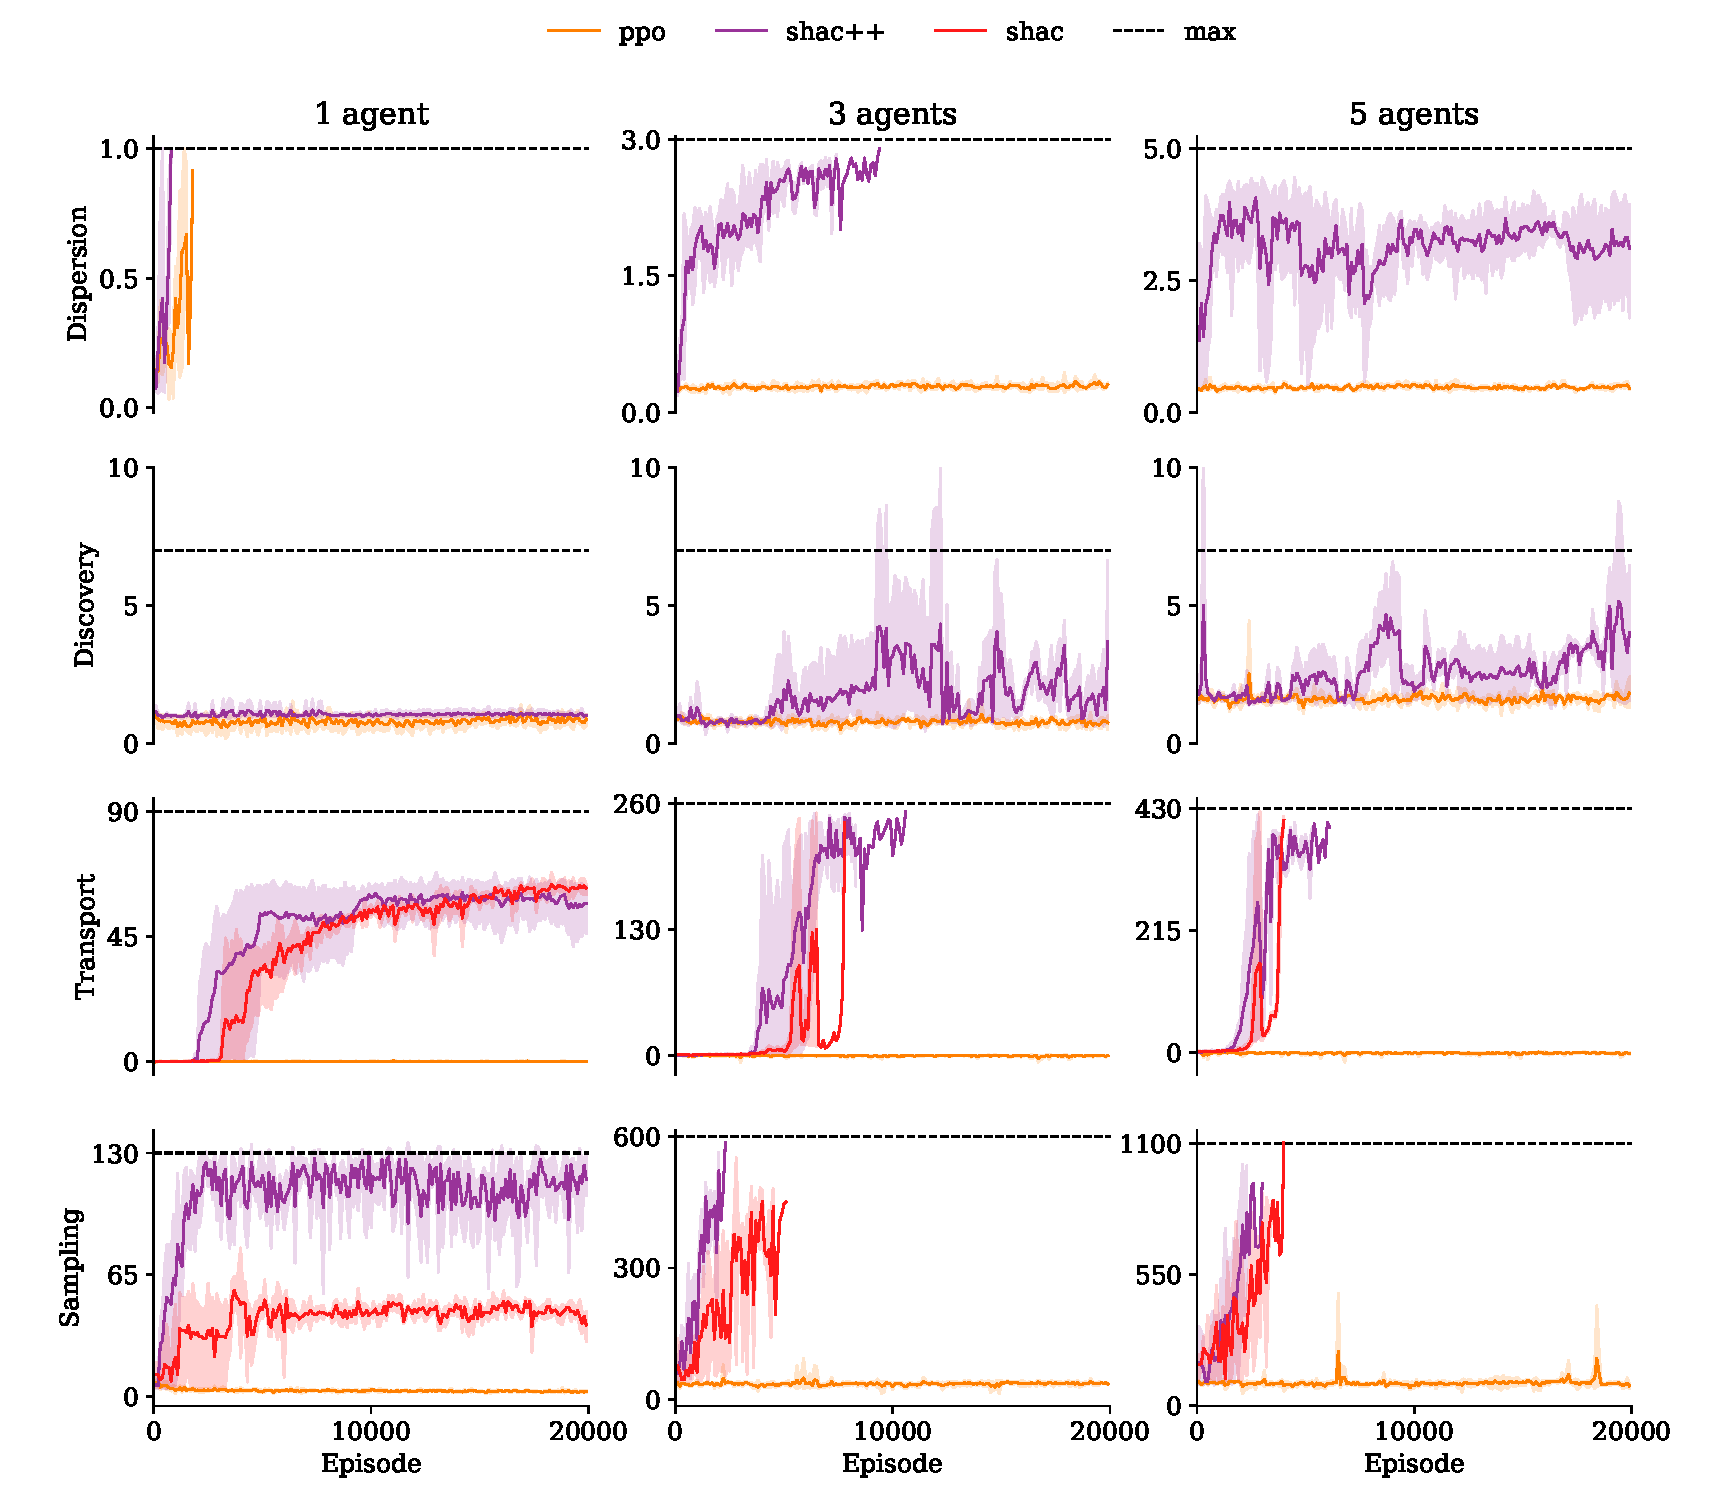
\includegraphics[width=0.75\textwidth]{figs/main-transformer.pdf}
    \caption{Performance comparison of \fname{}, PPO/MAPPO, and SHAC across different scenarios (Dispersion, Transport, Discovery, and Sampling) using the Transformer architecture for multi-agent settings and the MLP architecture for single-agent settings. The results show the mean and standard deviation of rewards over 3 runs. For results using the MLP architecture in all scenarios, refer to \Cref{apx:fig:experiments-mlp}.}%
    \label{fig:experiments}
\end{figure*}

\begin{table}[t]
    \centering
    \input tables/max.tex
    \vspace{0.2cm}
    \caption{Normalized rewards (relative to the best performing model) for the different scenarios. Best results are in bold. \textsc{D} stands for Dispersion, \textsc{T} for Transport, \textsc{Di} for Discovery, and \textsc{S} for Sampling.}\label{tab:max-rewards}.
\end{table}


